\documentclass[11pt]{article}
\usepackage{colacl}
\usepackage{graphicx}
\usepackage{listings}
\sloppy

\title{Report for COMP90025 Assignment 1 Task A \\
  \large Implementation of paralled \\
  Floyd-Warshall algorithm}

\author{Zichun Zhu \texttt{784145} \and Yijian Zhang \texttt{806676}}

\begin{document}
\maketitle

\section{Introduction}
The focus of this report is implementing an paralled solution for the all-pairs shortest path problem(APSP). Our aim is to find the diameter, which is the maximum of the shortest path lengths between all pairs of nodes of a graph. 

There are some exsited algorithms to solve APSP problem, such as the Dijkastra and the Floyd-Warshall (FW) algorithms\cite{albalawi2013task}. Considering the structures of the algorithms, the squential Floyd-Wallshall's algorithm has explicitly three nested loops as in Listing \ref{lst:Code1}, which is more sutiable to make it parallel. We will focus on the FW algorithm.

\begin{lstlisting}[label={lst:Code1},caption={Sequantial standard FW algorithm.}, captionpos=b,basicstyle=\small]
for k = 1 to N
   for i = 1 to N
      for j = 1 to N
         dist[k][i][j] = 
         min(dist[k-1][i][j], 
         dist[k-1][i][k]
         + dist[k-1][k][j])
\end{lstlisting}

\section{FWI and FWT}
The code in Listing \ref{lst:Code1} is the standard FW algorithm, simply nested in three loops. The outtest variable k is the "via node" that the path goes through from i to j. Because the property, the standard algorithm has a dependence so that k has to be the outtest loop.

Sung-Chul had introduced an optimized FW algorithm in 2006\cite{Han:2006:PGA:1152154.1152189}. He devides an entire matrix of nodes(N*N) into smaller tiles(M*M)\footnote{A problem size of N, devided into M smaller problems with a problem size of L.}, called tiled Floyd-Warshall(FWT). Then iterative Floyd-Warshall devided L again into smaller  submatrixes with problem size L. Note that such algorithm does not decrease the time complexity of APSP problems, but it improves the data reusage and breaks the inner dependency of i, j, and k. In more percific there are four phases shown in Figure \ref{fig:phases}. In the phase 4 the three submatrix are not overclapped, which means they are all independent. In this case, i, j, k can swap positions freely. Moreover, after FWT splits the entire matrix into submatrixes, the iteratice FW(FWI) algorithm  can be used. It devides the submatrix again by size of U.
\begin{figure}
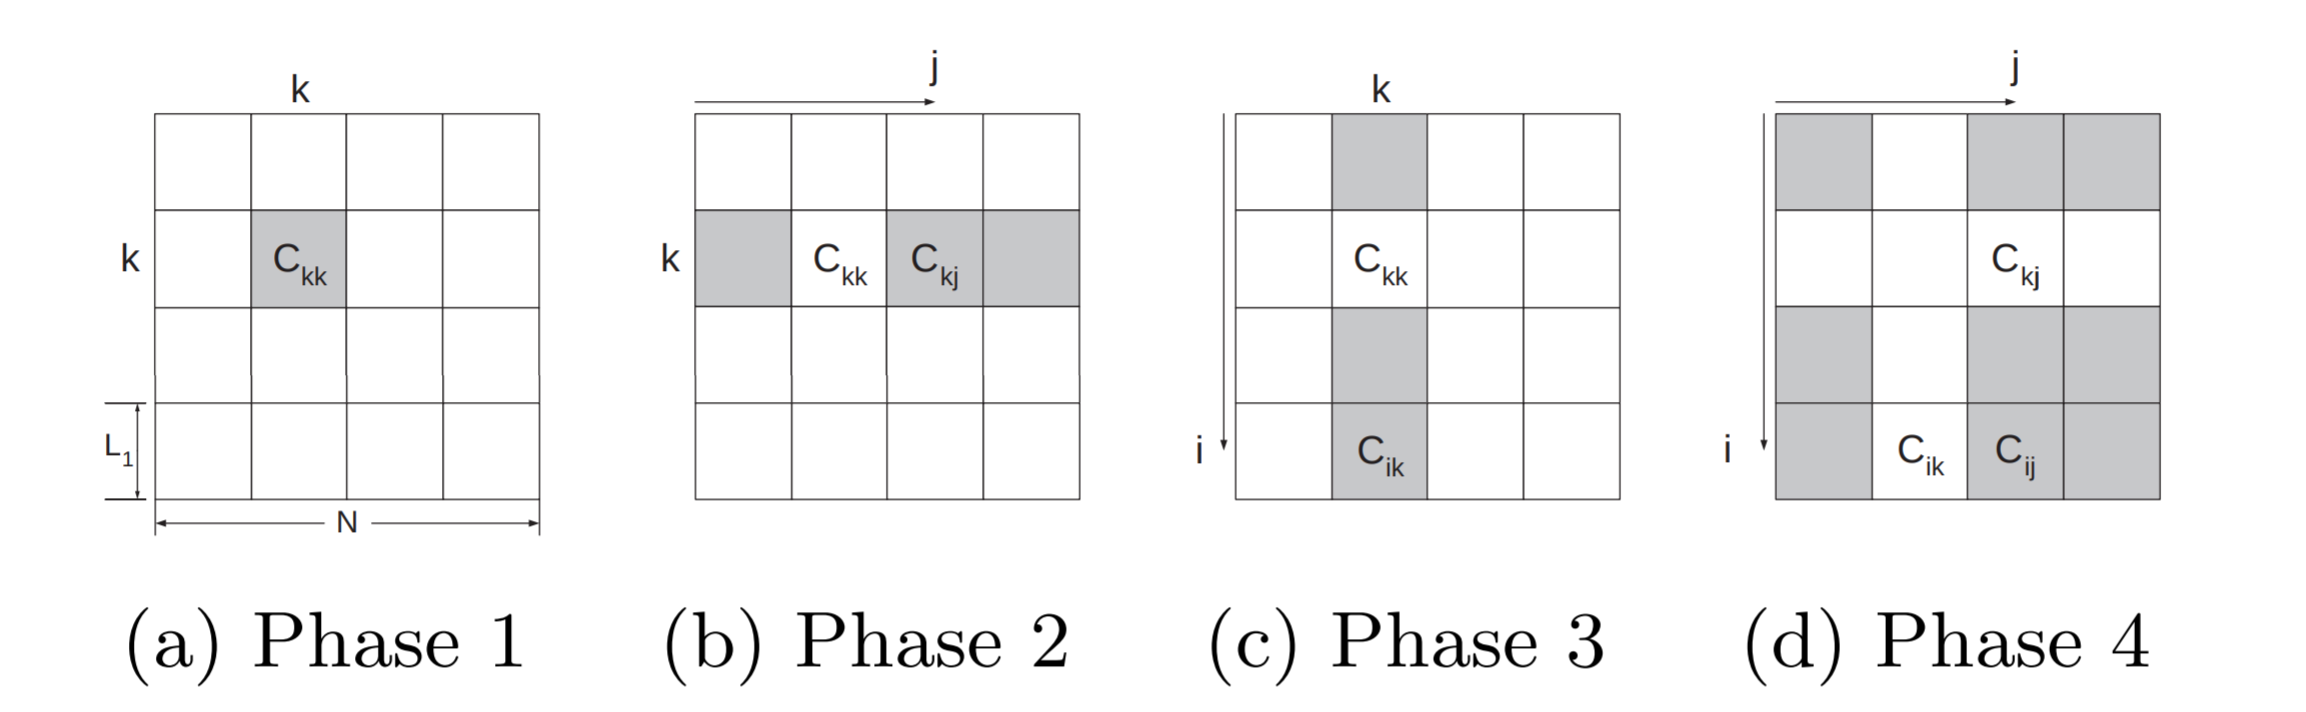
\includegraphics[width=3.05in]{FWT_phases}
	\caption{Four phases in FWT\cite{Han:2006:PGA:1152154.1152189}}
    \label{fig:phases}
\end{figure}


\section{Result}

\begin{figure}
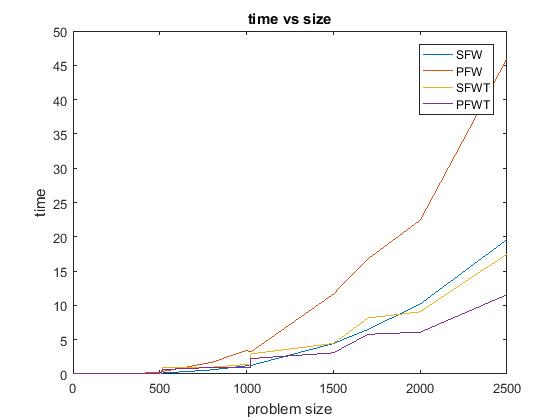
\includegraphics[width=3.05in]{plot}
	\caption{Fime vs problem size.\cite{Han:2006:PGA:1152154.1152189}}
    \label{fig:plot}
\end{figure}

Figure \ref{fig:plot} clearly shows that the tiled Floyd-Warshall spend less time, plus the OpenMP optimization. It proformace better than the standard algorithm. But there is a interesting point that in -O3 the paralled standard FW is even worth than sequential standard FW. The reason is not clear for us, but we condistered is the the limite of bandwidth of the memory.


\begin{table}[h]
 \begin{center}
\begin{tabular}{|l|l|}

      \hline
      Corpus & Features\\
      \hline\hline
      AAA & 1M words\\
      BBB & spoken corpus (expensive)\\
      CCC & 2M words\\
        & free (to academics)\\
      \hline

\end{tabular}
\caption{The caption of the table}\label{table1}
 \end{center}
\end{table}

\bibliographystyle{abbrv}
\bibliography{bib}

\end{document}
